% Author: Izaak Neutelings (September 2021)
% Inspiration:
%   https://www.asimovinstitute.org/neural-network-zoo/
%   https://www.youtube.com/watch?v=aircAruvnKk&list=PLZHQObOWTQDNU6R1_67000Dx_ZCJB-3pi&index=1
\documentclass[border=3pt,tikz]{standalone}
\usepackage{amsmath} % for aligned
%\usepackage{amssymb} % for \mathbb
\usepackage{tikz}
%\usepackage{etoolbox} % for \ifthen
\usepackage{listofitems} % for \readlist to create arrays
\usetikzlibrary{arrows.meta} % for arrow size
\usepackage[outline]{contour} % glow around text
\contourlength{1.4pt}

\tikzset{>=latex} % for LaTeX arrow head
\usepackage{xcolor}
\colorlet{myred}{red!80!black}
\colorlet{myblue}{blue!80!black}
\colorlet{mygreen}{green!60!black}
\colorlet{myorange}{orange!70!red!60!black}
\colorlet{mydarkred}{red!30!black}
\colorlet{mydarkblue}{blue!40!black}
\colorlet{mydarkgreen}{green!30!black}
\tikzstyle{node}=[thick,circle,draw=myblue,minimum size=22,inner sep=0.5,outer sep=0.6]
\tikzstyle{node in}=[node,green!20!black,draw=mygreen!30!black,fill=mygreen!25]
\tikzstyle{node hidden}=[node,blue!20!black,draw=myblue!30!black,fill=myblue!20]
\tikzstyle{node convol}=[node,orange!20!black,draw=myorange!30!black,fill=myorange!20]
\tikzstyle{node out}=[node,red!20!black,draw=myred!30!black,fill=myred!20]
\tikzstyle{connect}=[thick,mydarkblue] %,line cap=round
\tikzstyle{connect arrow}=[-{Latex[length=4,width=3.5]},thick,mydarkblue,shorten <=0.5,shorten >=1]
\tikzset{ % node styles, numbered for easy mapping with \nstyle
  node 1/.style={node in},
  node 2/.style={node hidden},
  node 3/.style={node out},
}
\def\nstyle{int(\lay<\Nnodlen?min(2,\lay):3)} % map layer number onto 1, 2, or 3

\begin{document}

% NEURAL NETWORK activation
% https://www.youtube.com/watch?v=aircAruvnKk&list=PLZHQObOWTQDNU6R1_67000Dx_ZCJB-3pi&index=1
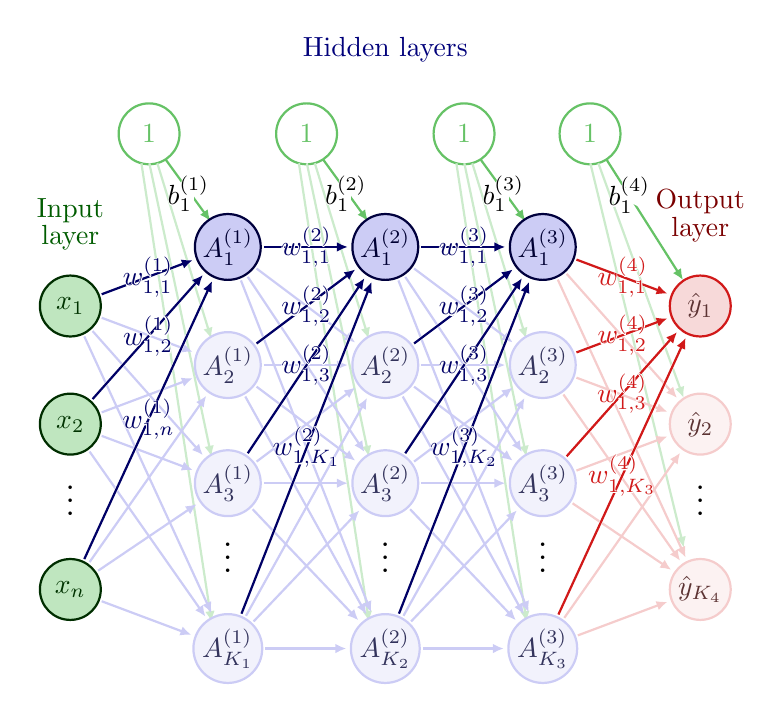
\begin{tikzpicture}[x=2cm,y=1.5cm]
  \message{^^JNeural network activation}
  \def\NI{3} % number of nodes in input layers
  \def\NH{4} % number of nodes in hidden layer 1
  \def\NHto{4} % number of nodes in hidden layer 2
  \def\NHtre{4} % number of nodes in hidden layer 3
  \def\NO{3} % number of nodes in output layers
  \def\yshift{0.4} % shift last node for dots
  
  % INPUT LAYER
  \foreach \i [evaluate={\c=int(\i==\NI); \y=\NI/2-\i-\c*\yshift; \index=(\i<\NI?int(\i):"n");}]
              in {1,...,\NI}{ % loop over nodes
    \node[node in,outer sep=0.6] (NI-\i) at (0,\y) {$x_{\index}$};
  }
  
    % BIAS TERM 1
  \node[node, above=200,align=center,mygreen!60!] at (\NI-2.5,1-4) {$1$};
  \draw[connect arrow,mygreen!60!] (0.6,1.75) -- (0.9,1.2);
  \draw[connect arrow,mygreen!20!] (0.55,1.72) -- (0.9,0.2);
  \draw[connect arrow,mygreen!20!] (0.5,1.72) -- (0.9,-0.8);
  \draw[connect arrow,mygreen!20!] (0.45,1.72) -- (0.9,-2.2);
  %\draw[connect arrow] (\NO-0.25,\NO+0.24) -- (\NO,-0.6);
  \draw[connect,white,line width=4] (0.75,1.75) -- (0.75,1.2);
  \node[] at (1-0.25,1.45) {\contour{white}{$b_{1}^{(1)}$}};
  
    % HIDDEN LAYER
  \foreach \i [evaluate={\c=int(\i==\NH); \y=(\NH/2-\i-\c*\yshift); \index=(\i<\NH?int(\i):"K_1");}]
    in {\NH,...,1}{ % loop over nodes
    \ifnum\i=1 % high-lighted node
      \node[node hidden]
        (NH-\i) at (1,\y) {$A_{\index}^{(1)}$};
      \foreach \j [evaluate={\index=(\j<\NI?int(\j):"n");}] in {1,...,\NI}{ % loop over nodes in previous layer
        \draw[connect arrow,white,line width=1.2] (NI-\j) -- (NH-\i);
        \draw[connect arrow] (NI-\j) -- (NH-\i)
          node[pos=0.50] {\contour{white}{$w_{1,\index}^{(1)}$}};
      }
    \else % other light-colored nodes
      \node[node,blue!20!black!80,draw=myblue!20,fill=myblue!5]
        (NH-\i) at (1,\y) {$A_{\index}^{(1)}$};
      \foreach \j in {1,...,\NI}{ % loop over nodes in previous layer
        %\draw[connect arrow,white,line width=1.2] (NI-\j) -- (NO-\i);
        \draw[connect arrow,myblue!20] (NI-\j) -- (NH-\i);
      }
    \fi
  }
  
      % BIAS TERM 2
  \node[node, above=200,align=center,mygreen!60!] at (\NH-2.5,1-4) {$1$};
  \draw[connect arrow,mygreen!60!] (1.6,1.75) -- (1.9,1.2);
  \draw[connect arrow,mygreen!20!] (1.55,1.72) -- (1.9,0.2);
  \draw[connect arrow,mygreen!20!] (1.5,1.72) -- (1.9,-0.8);
  \draw[connect arrow,mygreen!20!] (1.45,1.72) -- (1.9,-2.2);
  %\draw[connect arrow] (\NO-0.25,\NO+0.24) -- (\NO,-0.6);
  \draw[connect,white,line width=4] (1.75,1.75) -- (1.75,1.2);
  \node[] at (1.75,1.45) {\contour{white}{$b_{1}^{(2)}$}};
  
  % HIDDEN LAYER 2
  \foreach \i [evaluate={\c=int(\i==\NHto); \y=(\NHto/2-\i-\c*\yshift); \index=(\i<\NHto?int(\i):"K_2");}]
    in {\NHto,...,1}{ % loop over nodes
    \ifnum\i=1 % high-lighted node
      \node[node hidden]
        (NHto-\i) at (1+1,\y) {$A_{\index}^{(2)}$};
      \foreach \j [evaluate={\index=(\j<\NH?int(\j):"K_1");}] in {1,...,\NH}{ % loop over nodes in previous layer
        \draw[connect arrow,white,line width=1.2] (NH-\j) -- (NHto-\i);
        \draw[connect arrow] (NH-\j) -- (NHto-\i)
          node[pos=0.50] {\contour{white}{$w_{1,\index}^{(2)}$}};
      }
    \else % other light-colored nodes
      \node[node,blue!20!black!80,draw=myblue!20,fill=myblue!5]
        (NHto-\i) at (1+1,\y) {$A_{\index}^{(2)}$};
      \foreach \j in {1,...,\NH}{ % loop over nodes in previous layer
        %\draw[connect arrow,white,line width=1.2] (NI-\j) -- (NO-\i);
        \draw[connect arrow,myblue!20] (NH-\j) -- (NHto-\i);
      }
    \fi
  }
  
  % BIAS TERM 3
  \node[node, above=200,align=center,mygreen!60!] at (\NH-1.5,1-4) {$1$};
  \draw[connect arrow,mygreen!60!] (2.6,1.75) -- (2.9,1.2);
  \draw[connect arrow,mygreen!20!] (2.55,1.72) -- (2.9,0.2);
  \draw[connect arrow,mygreen!20!] (2.5,1.72) -- (2.9,-0.8);
  \draw[connect arrow,mygreen!20!] (2.45,1.72) -- (2.9,-2.2);
  %\draw[connect arrow] (\NO-0.25,\NO+0.24) -- (\NO,-0.6);
  \draw[connect,white,line width=4] (2.75,1.75) -- (2.75,1.2);
  \node[] at (2.75,1.45) {\contour{white}{$b_{1}^{(3)}$}};
  
  % HIDDEN LAYER 3
  \foreach \i [evaluate={\c=int(\i==\NHtre); \y=(\NHtre/2-\i-\c*\yshift); \index=(\i<\NHtre?int(\i):"K_3");}]
    in {\NHtre,...,1}{ % loop over nodes
    \ifnum\i=1 % high-lighted node
      \node[node hidden]
        (NHtre-\i) at (1+2,\y) {$A_{\index}^{(3)}$};
      \foreach \j [evaluate={\index=(\j<\NHto?int(\j):"K_2");}] in {1,...,\NHto}{ % loop over nodes in previous layer
        \draw[connect arrow,white,line width=1.2] (NHto-\j) -- (NHtre-\i);
        \draw[connect arrow] (NHto-\j) -- (NHtre-\i)
          node[pos=0.50] {\contour{white}{$w_{1,\index}^{(3)}$}};
      }
    \else % other light-colored nodes
      \node[node,blue!20!black!80,draw=myblue!20,fill=myblue!5]
        (NHtre-\i) at (1+2,\y) {$A_{\index}^{(3)}$};
      \foreach \j in {1,...,\NHto}{ % loop over nodes in previous layer
        %\draw[connect arrow,white,line width=1.2] (NI-\j) -- (NO-\i);
        \draw[connect arrow,myblue!20] (NHto-\j) -- (NHtre-\i);
      }
    \fi
  }
  
    % BIAS TERM 4
  \node[node, above=200,align=center,mygreen!60!] at (\NH-0.7,1-4) {$1$};
  \draw[connect arrow,mygreen!60!] (3.4,1.75) -- (3.9,0.7);
  \draw[connect arrow,mygreen!20!] (3.35,1.72) -- (3.9,-0.3);
  \draw[connect arrow,mygreen!20!] (3.3,1.72) -- (3.9,-1.57);
  %\draw[connect arrow] (\NO-0.25,\NO+0.24) -- (\NO,-0.6);
  \draw[connect,white,line width=4] (3.45,1.5) -- (3.9,1.2);
  \node[] at (3.55,1.44) {\contour{white}{$b_{1}^{(4)}$}};
  
  % OUTPUT LAYER
  \foreach \i [evaluate={\c=int(\i==\NO); \y=(\NO/2-\i-\c*\yshift); \index=(\i<\NO?int(\i):"K_{4}");}]
    in {\NO,...,1}{ % loop over nodes
    \ifnum\i=1 % high-lighted node
      \node[node hidden,red!20!black!80,draw=myred!90,fill=myred!15]
        (NO-\i) at (1+3,\y) {$\hat{y}_{\index}$};
      \foreach \j [evaluate={\index=(\j<\NHto?int(\j):"K_3");}] in {1,...,\NHtre}{ % loop over nodes in previous layer
        \draw[connect arrow,white,line width=1.2] (NHtre-\j) -- (NO-\i);
        \draw[connect arrow,myred!90] (NHtre-\j) -- (NO-\i)
          node[pos=0.50] {\contour{white}{$w_{1,\index}^{(4)}$}};
      }
    \else % other light-colored nodes
      \node[node,red!20!black!80,draw=myred!20,fill=myred!5]
        (NO-\i) at (1+3,\y) {$\hat{y}_{\index}$};
      \foreach \j in {1,...,\NHtre}{ % loop over nodes in previous layer
        %\draw[connect arrow,white,line width=1.2] (NI-\j) -- (NO-\i);
        \draw[connect arrow,myred!20] (NHtre-\j) -- (NO-\i);
      }
    \fi
  }
  
  % DOTS
  \path (NI-\NI) --++ (0,1+\yshift) node[midway,scale=1.2] {$\vdots$};
  \path (NH-\NH) --++ (0,1+\yshift) node[midway,scale=1.2] {$\vdots$};
  \path (NHto-\NHto) --++ (0,1+\yshift) node[midway,scale=1.2] {$\vdots$};
  \path (NHtre-\NHtre) --++ (0,1+\yshift) node[midway,scale=1.2] {$\vdots$};
  \path (NO-\NO) --++ (0,1+\yshift) node[midway,scale=1.2] {$\vdots$};
  
  % LABELS
  \node[above=5,align=center,mygreen!60!black] at (NI-1.90) {Input\\[-0.2em]layer};
  \node[above=8,align=center,myblue!60!black] at (2,2.3) {Hidden layers};
  \node[above=8,align=center,myred!60!black] at (NO-1.90) {Output\\[-0.2em]layer};
  
\end{tikzpicture}

\end{document}